\section{Newton's Third Law}

\subsection{Interacting Objects}

\begin{figure}
    \centering
    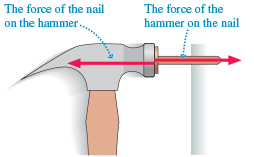
\includegraphics[width=0.4\textwidth]{../figures/hammer-on-nail.png}
    \caption{The hammer and nail are interacting with each other.}%
    \label{fig:hammer-nail-interaction}
\end{figure}

Figure~%
\ref{fig:hammer-nail-interaction} shows a hammer hitting a nail.  The
hammer exerts a force on the nail.  At the same time the nail exerts a
force on the hammer.

\begin{figure}
    \centering
    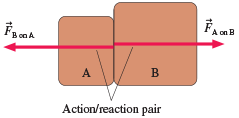
\includegraphics[width=0.4\textwidth]{../figures/action-reaction-pair.png}
    \caption{An action/reaction pair of forces.}%
    \label{fig:action-reaction-pair}
\end{figure}

If object A exerts a force
$
    \vec{F}_{\mathrm{~A~on~B}}
$ on object B, then object B exerts a force
$
    \vec{F}_{\mathrm{~B~on~A}}
$ on object A. This pair of forces, shown in Figure~%
\ref{fig:action-reaction-pair}, is called an \textbf{action/reaction
pair}.

\subsection{Propulsion}

The friction force
$
    \vec{f}_P
$ (force of surface on person) is an example of propulsion.  If you try
to walk accross a frictionless floor, your foot slips and slides \emph{backward}.
In order for you to walk, the floor needs have friction so that your
foot \emph{sticks} to the floor as you straighten your leg, moving your
body forward.  The friction that prevents slipping is \emph{static}
friction.  The static friction force
$
    \vec{f}_P
$ has to point in the \emph{forward} direction to prevent your foot from
slipping backward.  It is this forward-directed static friction that
propels you forward!  The force of your foot on the floor, and the other
half of the action/reaction pair, is in the opposite direction.  Figure~%
\ref{fig:propulsion} shows examples of propulsion.

\begin{figure}
    \centering
    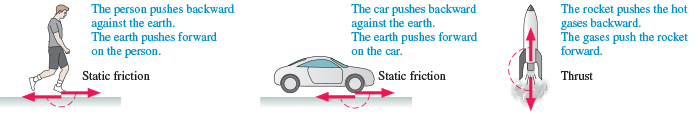
\includegraphics[width=\textwidth]{../figures/propulsion-examples.png}
    \caption{Propulsion examples.}%
    \label{fig:propulsion}
\end{figure}

\subsection{Newton's Third Law}

\begin{theorem}[Newton's Third Law]
    Every force occurs as one member of an action/reaction pair of
    forces.
    \begin{enumerate}
        \item
            The two members of an action/reaction pair act on two \emph{different}
            objects.
        \item
            The two members of an action/reaction pair are equal in
            magnitude but opposite in direction:
            $
                \vec{F}_{\mathrm{~A~on~B}} = -\vec{F}_{\mathrm{~B~on~A}}
            $
    \end{enumerate}
    \label{theo:newtons-third-law}
\end{theorem}
\begin{remark}
    All forces are just an \emph{interaction} between two objects.
\end{remark}

\begin{figure}
    \centering
    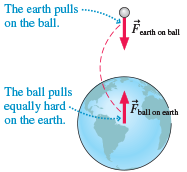
\includegraphics[width=0.4\textwidth]{../figures/ball-dropping-action-reaction.png}
    \caption{The action/reaction forces of a ball and the earth are
    equal in magnitude.}%
    \label{fig:ball-dropping}
\end{figure}

Figure~%
\ref{fig:ball-dropping} shows a ball dropping.  If the magnitude of the
forces
$
    \vec{F}_{\mathrm{~earth~on~ball}}
$ and
$
    \vec{F}_{\mathrm{~ball~on~earth}}
$ are equal, then why does the earth not ``fly up'' to meet the ball?
This is because while the magnitude of the forces are equal, \textbf{the
accelerations are not}.

\subsection{Ropes and Pulleys}

\begin{figure}
    \centering
    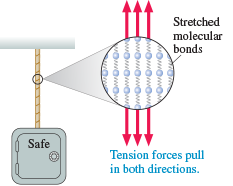
\includegraphics[width=0.6\textwidth]{../figures/tension-inside-rope.png}
    \caption{Tension inside rope are due to stretching the spring-like
    molecules.}%
    \label{fig:tension-inside}
\end{figure}

Figure~%
\ref{fig:tension-inside} shows a heavy safe hanging from a rope, placing
the rope under tension.  If you cut the rope, the safe and the lower
portion of the rope will fall.  Thus, there must be a force \emph{within}
the rope by which the upper portion of the rope pulls upward on the
lower portion to prevent it from falling.
\begin{remark}
    In this scenario, tension pulls equally \emph{in both directions}.
\end{remark}

\begin{Exercise}[title={Pulling a rope}, label={ex:pulling-a-rope}
    origin={Knight}]
    \begin{minipage}[t]
        {0.4\linewidth}
        \vspace{-2ex} 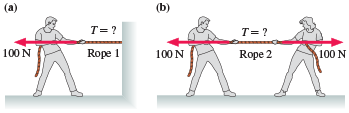
\includegraphics{../figures/wall-rope-vs-human-rope.png}
        \captionof{figure}{Compare the tensions.}%
        \label{fig:wall-rope-vs-human-rope}
    \end{minipage}

    Figure~%
    \ref{fig:wall-rope-vs-human-rope}a shows a person pulling with a
    $
        \qty{100}{\newton}
    $ on a rope attached to the wall.  Figure~%
    \ref{fig:wall-rope-vs-human-rope}b shows two humans pulling the rope
    on opposite ends with a
    $
        \qty{100}{\newton}
    $ of force.  Is the tension in the second rope larger than, smaller
    than, or the same as the first rope?
\end{Exercise}

\begin{Answer}
    \begin{proof}
        Let
        $
            \vec{F}_{\mathrm{~P~on~R}} = \qty{100}{\newton}
        $ be the force of the person on the rope in Figure~%
        \ref{fig:wall-rope-vs-human-rope}a.  We know from Newton's Third
        Law, Theorem~%
        \ref{theo:newtons-third-law}, forces
        \begin{equation}
            \vec{F}_{\mathrm{~P~on~R}} = -\vec{F}_{\mathrm{~R~on~P}}
        \end{equation}
        and are an action/reaction pair.  Similarly for force
        $
            \vec{F}_{\mathrm{~R~on~W}}
        $%
        , rope on wall:
        \begin{equation}
            \vec{F}_{\mathrm{~R~on~W}}=-\vec{F}_{\mathrm{~W~on~R}}
        \end{equation}
        because the force is in static equilibrium, that is the rope is
        not accelerating and is at rest.  Thus
        \begin{equation}
            F_{\mathrm{~P~on~R}} = F_\mathrm{~R~on~P} = F_{\mathrm{~R~on~W}}
            = F_{\mathrm{~W~on~R}} = \qty{100}{\newton}
        \end{equation}

        Forces
        $
            \arpair{R}{P}
        $ and
        $
            \arpair{P}{R}
        $ are the pulling forces exerted by the rope and what we \emph{mean}
        by ``the tension in the rope''.  Thus the tension in the first
        rope is
        $
            \qty{100}{\newton}
        $%
        .

        For Figure~%
        \ref{fig:wall-rope-vs-human-rope}b, each person pulls wtih
        $
            \qty{100}{\newton}
        $ of force, so
        $
            \arpair{P1}{R}=\qty{100}{\newton}
        $ and
        $
            \arpair{P2}{R}=\qty{100}{\newton}
        $ where P1 and P2 are persons 1 and 2, and R is the rope.  Thus
        \begin{equation}
            \arpair{P1}{R} = \arpair{R}{P2} = \arpair{P2}{R} = \arpair{R}
            {P2} = \qty{100}{\newton}
        \end{equation}
        The tension in the rope--the pulling forces
        $
            \arpair{R}{P1}
        $ and
        $
            \arpair{R}{P2}
        $--is still
        $
            \qty{100}{\newton}
        $%
        !

    \end{proof}
\end{Answer}

\subsection{The Massless String Approximation}

\begin{figure}
    \centering
    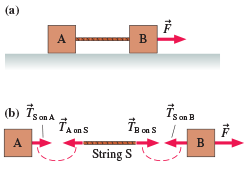
\includegraphics[width=0.4\textwidth]{../figures/two-blocks-accelerating-tension.png}
    \caption{Tension pulls forward on block A, backward on block B}%
    \label{fig:accelerating-tension}
\end{figure}

Figure~%
\ref{fig:accelerating-tension}a shows two connected blocks being pulled
by force
$
    \vec{F}
$%
.  Is the string's tension at the right end, where it pulls back on B,
the same as the tension at the left end where it pulls on A?

Figure~%
\ref{fig:accelerating-tension}b shows the horizontal forces acting on
the blocks and string.  The only forces acting on the string are
$
    \tarpair{A}{S}
$ and
$
    \tarpair{B}{S}
$%
, so Newton's First Law \emph{for the string} is
\begin{equation}
    \left(\vec{F}_{\mathrm{net}}\right)_x=\magtarpair{B}{S}-\magtarpair{A}
    {S}=m_sa_x
\end{equation}
where
$
    m_s
$ is the mass of the string.  If the string is accelerating, then the
tensions at the two ends \emph{cannot} be the same, that is
$
    \magtarpair{B}{S} > \magtarpair{A}{S}
$%
.

However, if the mass of the string or rope is much less the masses of
the objects it connects, we can adopt the \textbf{massless string
approximation}:
\begin{align}
    \left(\vec{F}_{\mathrm{net}}\right)_x = \magtarpair{B}{S}-\magtarpair
    {A}{S} &= m_sa_x \\
    \lim_{a_x \to 0}\magtarpair{B}{S}-\magtarpair{A}{S} &= m_sa_x \\
    \magtarpair{B}{S}-\magtarpair{A}{S} &= 0 \\
    \magtarpair{B}{S} &= \magtarpair{A}{S}
\end{align}
\begin{remark}
    Even though
    $
        \magtarpair{B}{S} = \magtarpair{A}{S}
    $ and the net force of the string is zero, because the mass is zero
    the acceleration can still be anything.
\end{remark}

Look again at%
\ref{fig:accelerating-tension}.  If
$
    \magtarpair{B}{S} = \magtarpair{A}{S}
$ then
\begin{equation}
    \tarpair{S}{A} = -\tarpair{S}{B}
\end{equation}

That is, the force on block A is equal and opposite to the force on
block B. The forces act as if they were action/reaction pair forces.
\begin{remark}
    A geometric constraint of massless strings is that they do not
    stretch.  If A moves three meters, so will B. Thus their
    accelerations are also the same.
\end{remark}
\begin{Exercise}[title={Comparing two tensions} origin={Knight}]
    \begin{minipage}[t]
        {0.4\linewidth}
        \vspace{-2ex} 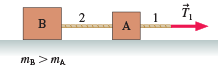
\includegraphics[width=\textwidth]{../figures/comparing-two-tensions.png}
        \captionof{figure}{Block A and B are pulled across a
        frictionless table by massless strings.}%
        \label{fig:comparing-two-tensions}
    \end{minipage}
    Blocks A and B in Figure~%
    \ref{fig:comparing-two-tensions} are connected by massless string 2
    and pulled across a frictionless table by massless string 1.  B has
    a larger mass than A. Is the tension in string 2 larger than,
    smaller than, or equal to the tension in string 1?
\end{Exercise}
\begin{Answer}
    \begin{minipage}[t]
        {0.4\linewidth}
        \vspace{-2ex} 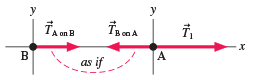
\includegraphics[width=\textwidth]{../figures/tension-comparison-model.png}
        \captionof{figure}{The horizontal forces on block A and B.}%
        \label{fig:tension-comparison-model}
    \end{minipage}
    Here we model the problem as Figure~%
    \ref{fig:tension-comparison-model}

    From Newton's Third Law, Theorem~%
    \ref{theo:newtons-third-law}, we define
    \begin{equation}
        T_2\coloneqq \magtarpair{A}{B} = \magtarpair{B}{A}
    \end{equation}
    where
    $
        T_2
    $ is the tension in string 2.  From Newton's Second Law, the net
    force on A is
    \begin{equation}
        \fnetx[A]=T_1-\magtarpair{B}{A}=T_1-T_2=m_Aa_{Ax}
    \end{equation}
    The blocks are accelerating to the right, making
    $
        a_x > 0
    $%
    , thus
    \begin{equation}
        T_1 > T_2
    \end{equation}
\end{Answer}

\subsection{Pulleys}

\begin{figure}
    \centering
    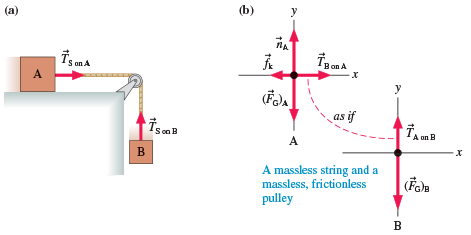
\includegraphics[width=\textwidth]{../figures/pulley-example-model.png}
    \caption{Blocks A and B are connected by a string that passes over a
    pulley}%
    \label{fig:pulley-example}
\end{figure}

Figure~%
\ref{fig:pulley-example} shows a situation in which block B, as it
falls, drags block A across the table.  If we assume that
\begin{enumerate}
    \item
        The string \emph{and} the pulley are massless
    \item
        There is no friction where the pulley turns on its axle
\end{enumerate}
Then no net force is needed to accelerate or turn the pulley.  Thus,
\textbf{the tension in a massless string remains constant as it passes
over a massless, frictionless pulley}

For massless ropes or strings and massless, frictionless pulleys:
\begin{enumerate}
    \item
        If a force pulls on one end of a rope, the tension in the rope
        equals the magnitude of the pulling force.
    \item
        If two objects are connected by a rope, the tension is the same
        at both ends.
    \item
        If the rope passes over a pulley, the tension in the rope is
        unaffected.
\end{enumerate}

\subsection{Examples of Interacting-Objects Problems}

\begin{Exercise}[title={Placing a leg in traction}, origin={knight}]
    Serious fractures of the leg often need a stretching force to keep
    contracting leg muscles from forcing the broken bones together too
    hard.  This is done using a \emph{traction}, an arrangement of a
    rope, a weight, and pulleys as shown in Figure~%
    \ref{fig:leg-in-traction}.

    The rope must make the same angle on both sides of the pulley so
    that the net force on the leg is horizontal, but the angle can be
    adjusted to control the amount of traction.  The doctor has
    specified \SI{50}{\newton} of traction for this patient with a \SI{4.2}
    {\kilo\gram} hanging mass.  What is the proper angle?

    \begin{center}
        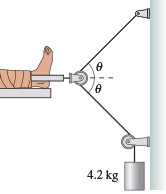
\includegraphics[totalheight=0.2\textheight]{../figures/leg-in-traction.png}
        \captionof{figure}{A leg in traction.}%
        \label{fig:leg-in-traction}
    \end{center}
\end{Exercise}
\begin{Answer}
    \begin{center}
        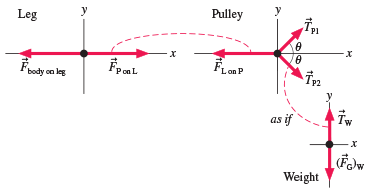
\includegraphics[totalheight=0.2\textheight]{../figures/leg-in-traction-model.png}
        \captionof{figure}{The free-body diagrams.}%
        \label{fig:leg-in-traction-model}
    \end{center}

    The x-component equation of Newton's second law for the pulley is
    \begin{align}
        \sum (F_{\mathrm{on~P}})_x &= T_{P1}\cos\theta -\magarpair{L}{P}
        \\
        &= 2T\cos\theta - \magarpair{L}{P} = 0
    \end{align}
    Thus, the correct angle for the ropes is
    \begin{equation}
        \theta = \arccos \left(\frac{\magarpair{L}{P}}{2T}\right)
    \end{equation}
    We know, from Newton's third law, that
    \begin{equation}
        \magarpair{L}{P} = \magarpair{P}{L} = \qty{50}{\newton}
    \end{equation}

    We can determine the tension force by analzying the weight.  It is
    also in equilibrium, so the upward tension force exactly balances
    the downward gravitational force:
    \begin{equation}
        T = (F_G)_W = m_Wg = (\qty{4.2}{\kilo\gram})(g) = \qty{41}{\newton}
    \end{equation}
    Thus the proper angle is
    \begin{equation}
        \theta = \arccos \left( \frac{\qty{50}{\newton}}{2(\qty{41}{\newton})}\right)=\ang
        {52}
    \end{equation}
\end{Answer}

\begin{Exercise}[title={The show must go on!}, origin={Knight}]
    A \SI{200}{\kilogram} set used in a play is stored in the loft above
    the stage.  The rope holding the set passes up and over a pulley,
    then is tied backstage.  The director tells a \SI{100}{\kilogram}
    stagehand to lower the set.  When he unties the rope, the set falls
    and the unfortunate man is hoisted into the loft.  What is the
    stagehand's acceleration?
\end{Exercise}
\begin{Answer}
    \begin{center}
        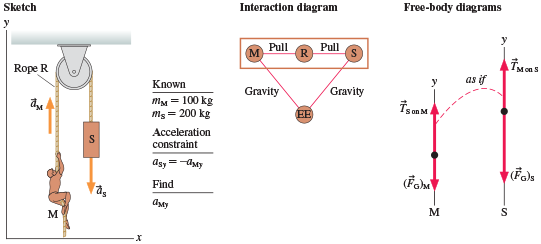
\includegraphics[totalheight=0.2\textheight]{../figures/stagehand-pictorial.png}
        \captionof{figure}{Stagehand pictorial representation}%
        \label{fig:stagehand-model}
    \end{center}

    In massless string approximation, the acceleration of the set and
    the man will be the same.  Thus, using Newton's second law we see
    that:
    \begin{align}
        \sum \left(F_{\mathrm{on~M}}\right)_y &= \magarpair{S}{M} = m_M
        a_{My} \sum \left(F_{\mathrm{on~S}}\right)_y &= \magarpair{M}{S}
        - m_sg = m_s a_ {Sy} = -m_s a_{My}
    \end{align}
    Newton's third law is
    \begin{equation}
        \magarpair{M}{S}=\magarpair{S}{M}=T
    \end{equation}
    where we can drop the subscripts and call the tension simply
    $
        T
    $%
.    The two second-law equations can be written
    \begin{align}
        T-m_Mg &= m_Ma_{my} T-M_sg &= -m_sa_{My}
    \end{align}
\end{Answer}
